\section{Kabel}

\subsection{Resistanzbelag}
\vspace{-2em}
\begin{gather*}
    F_\vartheta = 1+\alpha \cdot(\vartheta_{max} - 20\degree C)\\
    R'_b=R'_=\cdot F_\vartheta \cdot F_S \cdot F_P
\end{gather*}
$F_S$: Skineffekt (F35) \\
$F_P:$ Proximity-Effekt (F37)

\subsection{Reaktanzbelag}
Metallmantel keine Schirmung! Für $D$ nicht $\gg r$!\\
\indent $r:$ Radius des (Innen-)Leiters, nicht vom Mantel!

\textbf{Wechselstromkabel}
\begin{equation*}
    X_{b}' = \pi \left( 4 \ln \left( \frac{D}{r} -1\right) +1 \right) \cdot 10 ^{-2}   \left[\frac{\Omega}{km}\right]
\end{equation*}

\textbf{Einfach-Drehstromkabel}
\begin{equation*}
    X_{b}' = \pi \left( 2 \ln \left( \frac{D_{m}}{r} -1\right) +\frac{1}{2} \right) \cdot 10 ^{-2}   \left[\frac{\Omega}{km}\right]
\end{equation*}

\textbf{Doppel-Drehstromkabel}
\begin{equation*}
    X_{b}' = \pi \left( 2 \ln \left( \frac{D_{m} \cdot D_{L1L\RN{2}}}{r \cdot D_{L1L\RN{1}}} -1\right) +\frac{1}{2} \right) \cdot 10 ^{-2}   \left[\frac{\Omega}{km}\right]
\end{equation*}

\subsection{Suzeptanzbelag}
Metallmantel/-folie schirmt E-Feld ab!\\
\indent $B'_b$ gilt für $f=50Hz$\\
\indent $d:$ Schirmdurchmesser eines Leiters\\
\indent $D:$ Abstand zw. 2 Innenleiter

Bilder unbedingt einfügen !!

\textbf{Einleiter-/Dreimantel-/Radialfeldkabel}
\begin{gather*}
        C'_b = C'_{LE} = \frac{2\pi \cdot \varepsilon_0 \cdot \varepsilon_r}{ln \left( \frac{R}{r} \right)}\\
        B'_b= \omega C'_b  = \frac{17,47 \cdot \varepsilon_r}{ln \left(\frac{R}{r} \right)} \dfrac{\mu S}{km}
    \end{gather*}

\textbf{Wechselstromkabel - 2 Innenleiter}
\begin{gather*}
    C_{b}' = 2 \cdot C_{LE} + C_{LL} = \frac{\pi \cdot \varepsilon_{0} \cdot \varepsilon_{r}}{\ln \left( \left(\frac{D}{r}\right) \cdot \frac{(d^2 - D^2)}{(d^2 + D^2)} \right)}\\
   B'_b  = \frac{8,735 \cdot \varepsilon_{r}}{\ln \left( \left(\frac{D}{r}\right) \cdot \frac{(d^2 - D^2)}{(d^2 + D^2)} \right)} \dfrac{\mu S}{km}
\end{gather*}

\textbf{Einfach-Drehstromkabel - 3 Innenleiter}
\begin{gather*}
    C_{b}' = C_{LE} + 3 \cdot C_{LL} = \frac{4 \pi \cdot \varepsilon_{0} \cdot \varepsilon_{r}}{\ln \left( \left(\frac{D}{r}\right)^2 \cdot \frac{(0,75d^2 - D^2)^3}{(0,75d^2)^3 - (D^2)^3} \right)}\\
    B'_b = \frac{34,94 \cdot \varepsilon_{r}}{\ln \left( \left(\frac{D}{r}\right)^2 \cdot \frac{(0,75d^2 - D^2)^3}{(0,75d^2)^3 - (D^2)^3} \right)}
     \dfrac{\mu S}{km}
\end{gather*}
\indent keine Kopplung zum Nachbarsystem $B'_{\mathit{EDL}} = B'_{\mathit{DDL}}$

\subsection{Konduktanzbelag}
% \textcolor{dgreen}{Restleitfähigkeit der Isolierstoffe}
Ursache: Restleitfähigkeit der Isolierwerkstoffe\\ \indent bzw. Polarisationsverluste

\textbf{Verlustfaktor}
\begin{gather*}
    \tan \delta = \dfrac{I_{R}}{I_{C}} = \dfrac{1}{\omega C R} = \frac{G}{B}\\
    G_{b}' = B_{b}' \cdot \tan \delta = \omega C_{b}' \cdot \tan \delta
\end{gather*}
\begin{center}
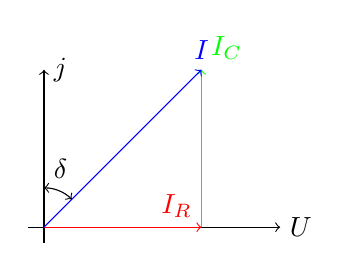
\begin{tikzpicture}
    \draw[->] (-0.2,0) -- (3,0)         node[right] {$\ul{U}$};
    \draw[->] (0,-0.2) -- (0,2)         node[right] {$j$};
    \draw[->, red] (0,0) -- (2,0)       node[above left] {$\ul{I}_{R}$};
    \draw[->, green] (2,0) -- (2,2)     node[above right] {$\ul{I}_{C}$};
    \draw[->, blue] (0,0) -- (2,2)      node[above] {$\ul{I}$};
    \draw[<->] (45:0.5) arc (45:90:0.5) node[above right] {$\delta$};
\end{tikzpicture}

\end{center}

\textbf{Dielektrische Verluste}
\begin{gather*}
    P_{Diel} = (\tan \delta \cdot \varepsilon_{r}) \cdot \omega \cdot C_{\mathit{Vakuum}} \cdot U^2 = G'_b\cdot U^2_{LE}
\end{gather*}
\indent $\tan \delta \cdot \varepsilon_{r}$: Verlustfaktor, siehe Tabelle \textbf{F43}

% \textcolor{red}{Werkstoff abhängige Verlustziffer}

\subsection{Leistung}
geg: $I_{max} , l , X'_b, G'_b$ \qquad ges: $P_{max}$
\begin{gather*}
    X_b = X'_b \cdot l \qquad G_b = G'_b \cdot l \\
    Q = 3 \cdot I^2_{max} \cdot X_b - 3 \cdot U^2_{LE} \cdot B_b\\
    P_{max} = \sqrt{S^2-Q^2}
\end{gather*}
